\documentclass[11pt]{article}
\usepackage[notes]{la}
\lamodule{6}{4}{The Gram--Schmidt Process}
\laxdoc{2.1}
\laxdoc{4.4}
\laxdoc{6.1}
\laxdoc{6.2}
\laxdoc{6.3}

\begin{document}

\section{The Gram--Schmidt Process}

\begin{guide}
Section 6.3 ended with two loose ends. The projection formula needs an \emph{orthogonal} basis, and we only had one when someone handed it to us or when we could build it by hand for a plane. And we did not know whether every subspace even has an orthogonal basis. This section settles both. Starting from any basis $\bv{x}_1,\dots,\bv{x}_p$, we build an orthogonal basis one vector at a time: keep $\bv{x}_1$, then replace $\bv{x}_2$ by what is left after removing its projection onto the line of $\bv{x}_1$, then replace $\bv{x}_3$ by what is left after removing its projection onto the plane of the first two, and so on. This is the \emph{Gram--Schmidt process}. Recording the bookkeeping in a matrix gives the \emph{QR factorization} $A=QR$, which writes a matrix as a product of a matrix with orthonormal columns and a triangular matrix.
\end{guide}

\textbf{By the end of this section you should be able to:}
\begin{itemize}
  \item apply the Gram--Schmidt process to independent vectors in $\R^n$ and check that the output is orthogonal and has the same span;
  \item recognise from a zero output that an input vector depends on the earlier ones;
  \item turn an orthogonal basis into an orthonormal basis, and use either to find a projection and a distance;
  \item explain why every subspace that is spanned by finitely many vectors has an orthogonal basis;
  \item find a QR factorization $A=QR$ and read the columns of $R$ as coordinates.
\end{itemize}

% ---------------------------------------------------------------------
\subsection*{One step: removing the part along an earlier vector}

At the end of Section 6.3 we replaced a second basis vector by its component orthogonal to the first (Example~\ref{6.3-ex:wrong}). Here is the same step in the plane, with the formula made explicit.

\begin{exmp}{Two vectors in the plane}{rtwo}
Let $\bv{x}_1=(3,1)$ and $\bv{x}_2=(1,2)$. They are not orthogonal, since $\bv{x}_1\cdot\bv{x}_2=5$. Keep $\bv{v}_1=\bv{x}_1$ and remove from $\bv{x}_2$ its projection onto the line $L=\Span\{\bv{v}_1\}$ (Definition~\ref{6.2-def:proj}). With $\bv{x}_2\cdot\bv{v}_1=5$ and $\bv{v}_1\cdot\bv{v}_1=10$,
\[
\proj_L\bv{x}_2=\tfrac{5}{10}(3,1)=(\tfrac32,\tfrac12),\qquad\bv{v}_2=\bv{x}_2-\proj_L\bv{x}_2=(1,2)-(\tfrac32,\tfrac12)=(-\tfrac12,\tfrac32).
\]
Check: $\bv{v}_1\cdot\bv{v}_2=-\tfrac32+\tfrac32=0$. \ $\checkmark$ The new pair spans the same plane: $\bv{v}_2=\bv{x}_2-\tfrac12\bv{x}_1$ and $\bv{x}_2=\tfrac12\bv{v}_1+\bv{v}_2$, so each pair is made from the other.
\end{exmp}

\begin{center}
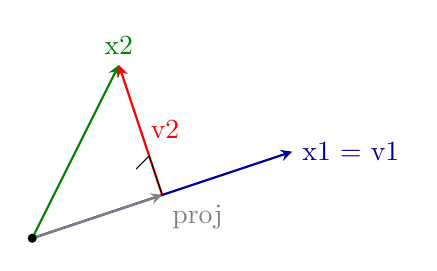
\begin{tikzpicture}[>=stealth,scale=1.1]
  \draw[->,thick,blue!60!black] (0,0)--(3,1) node[right] {x1 = v1};
  \draw[->,thick,green!50!black] (0,0)--(1,2) node[above] {x2};
  \draw[->,thick,gray] (0,0)--(1.5,0.5) node[below right] {proj};
  \draw[->,thick,red] (1.5,0.5)--(1,2) node[midway,right] {v2};
  \draw (1.5,0.5)--(1.35,0.95)--(1.2,0.8);
  \fill (0,0) circle (1.5pt);
\end{tikzpicture}
\end{center}

\noindent\textbf{Figure 1.} The vector $\bv{v}_2$ is $\bv{x}_2$ minus its projection onto the line of $\bv{v}_1$. It ends where $\bv{x}_2$ ends but starts on the line, at a right angle to it (drawn here from the foot of the projection).

\begin{exmp}{Two vectors in $\R^3$}{rthreetwo}
Let $\bv{x}_1=(1,1,1)$ and $\bv{x}_2=(1,2,4)$. Then $\bv{x}_2\cdot\bv{x}_1=7$ and $\bv{x}_1\cdot\bv{x}_1=3$, so
\[
\bv{v}_2=\bv{x}_2-\tfrac73\bv{x}_1=(1-\tfrac73,\ 2-\tfrac73,\ 4-\tfrac73)=(-\tfrac43,-\tfrac13,\tfrac53)=\tfrac13(-4,-1,5).
\]
Check: $\bv{x}_1\cdot\bv{v}_2=\tfrac13(-4-1+5)=0$. \ $\checkmark$ Again $\bv{x}_2=\tfrac73\bv{x}_1+\bv{v}_2$, so $\Span\{\bv{x}_1,\bv{x}_2\}=\Span\{\bv{x}_1,\bv{v}_2\}$: the plane has not changed, only the basis.
\end{exmp}

% ---------------------------------------------------------------------
\subsection*{The Gram--Schmidt process}

With three or more vectors, each new vector must be made orthogonal to \emph{all} the earlier new vectors, and the tool for that is the projection onto their span (Theorem~\ref{6.3-thm:decomp}).

\begin{thm}{The Gram--Schmidt Process}{gs}
Let $\bv{x}_1,\dots,\bv{x}_p$ be linearly independent vectors in $\R^n$. Define
\[
\bv{v}_1=\bv{x}_1,\qquad \bv{v}_k=\bv{x}_k-\frac{\bv{x}_k\cdot\bv{v}_1}{\bv{v}_1\cdot\bv{v}_1}\bv{v}_1-\cdots-\frac{\bv{x}_k\cdot\bv{v}_{k-1}}{\bv{v}_{k-1}\cdot\bv{v}_{k-1}}\bv{v}_{k-1}\qquad(k=2,\dots,p).
\]
Then for every $k$ from $1$ to $p$:
\begin{enumerate}[label=(\alph*),itemsep=1pt]
  \item $\bv{v}_1,\dots,\bv{v}_k$ are nonzero and orthogonal to one another;
  \item $\Span\{\bv{v}_1,\dots,\bv{v}_k\}=\Span\{\bv{x}_1,\dots,\bv{x}_k\}$.
\end{enumerate}
So $\bv{v}_1,\dots,\bv{v}_p$ is an orthogonal basis of $\Span\{\bv{x}_1,\dots,\bv{x}_p\}$. Moreover, the vectors $\bv{u}_k=\bv{v}_k/\lVert\bv{v}_k\rVert$ form an orthonormal basis of the same span.
\end{thm}

\begin{proof}
We use induction on $k$. For $k=1$, $\bv{v}_1=\bv{x}_1$ is nonzero because an independent set has no zero vector, and (b) is a statement about one vector.

Now let $k\ge2$ and assume (a) and (b) hold for $k-1$. Put $W=\Span\{\bv{x}_1,\dots,\bv{x}_{k-1}\}$. By assumption $\bv{v}_1,\dots,\bv{v}_{k-1}$ are nonzero and orthogonal, so they are independent (Theorem~\ref{6.2-thm:indep}), and they span $W$: an orthogonal basis of $W$. The sum subtracted from $\bv{x}_k$ in the definition of $\bv{v}_k$ is exactly the formula of Theorem~\ref{6.3-thm:decomp}(b) for this basis, so it is $\proj_W\bv{x}_k$ and
\[
\bv{v}_k=\bv{x}_k-\proj_W\bv{x}_k\quad\text{is in }W^{\perp}.
\]
(a)~Each $\bv{v}_j$ with $j<k$ is in $W$, hence $\bv{v}_k\cdot\bv{v}_j=0$. If $\bv{v}_k$ were $\bv{0}$, then $\bv{x}_k=\proj_W\bv{x}_k$ would lie in $W=\Span\{\bv{x}_1,\dots,\bv{x}_{k-1}\}$, and $\bv{x}_1,\dots,\bv{x}_k$ would be dependent, which they are not. So $\bv{v}_k\neq\bv{0}$.

(b)~Let $S=\Span\{\bv{x}_1,\dots,\bv{x}_k\}$. The vectors $\bv{v}_1,\dots,\bv{v}_{k-1}$ lie in $W$, and $W$ lies in $S$. Also $\bv{v}_k=\bv{x}_k-(\text{a combination of them})$ is in $S$. So
\[
\Span\{\bv{v}_1,\dots,\bv{v}_k\}\subseteq\Span\{\bv{x}_1,\dots,\bv{x}_k\}.
\]
Conversely $\bv{x}_k=\bv{v}_k+(\text{a combination of }\bv{v}_1,\dots,\bv{v}_{k-1})$ is in $\Span\{\bv{v}_1,\dots,\bv{v}_k\}$, and so are $\bv{x}_1,\dots,\bv{x}_{k-1}$, since they lie in $W=\Span\{\bv{v}_1,\dots,\bv{v}_{k-1}\}$. The two spans are equal.

Finally, $\bv{u}_k$ is a nonzero multiple of $\bv{v}_k$, so it spans the same line, and $\bv{u}_j\cdot\bv{u}_k=\dfrac{\bv{v}_j\cdot\bv{v}_k}{\lVert\bv{v}_j\rVert\lVert\bv{v}_k\rVert}=0$ for $j\neq k$, while $\lVert\bv{u}_k\rVert=1$ by Theorem~\ref{6.1-thm:scale}.
\end{proof}

\begin{proc}{Gram--Schmidt}{gsproc}
Given independent vectors $\bv{x}_1,\dots,\bv{x}_p$:
\begin{enumerate}[nosep]
  \item set $\bv{v}_1=\bv{x}_1$;
  \item for $k=2,\dots,p$: subtract from $\bv{x}_k$ its projection onto \emph{each earlier} $\bv{v}_j$ (not onto the earlier $\bv{x}_j$);
  \item if the result has fractions, multiply it by a convenient nonzero number (Pause and think~\ref{think:scale});
  \item check that the new vector is nonzero and has dot product $0$ with every earlier $\bv{v}_j$;
  \item for an orthonormal basis, divide each $\bv{v}_k$ by its length.
\end{enumerate}
\end{proc}

\begin{exmp}{Three vectors in $\R^3$}{rthree}
Let $\bv{x}_1=(1,1,-1)$, $\bv{x}_2=(3,-1,-1)$ and $\bv{x}_3=(3,1,2)$. Put $\bv{v}_1=\bv{x}_1$, so $\bv{v}_1\cdot\bv{v}_1=3$.

\emph{Step 2.} $\bv{x}_2\cdot\bv{v}_1=3-1+1=3$, so $\bv{x}_2-\tfrac33\bv{v}_1=(2,-2,0)$. This is twice $(1,-1,0)$; take $\bv{v}_2=(1,-1,0)$, with $\bv{v}_2\cdot\bv{v}_2=2$.

\emph{Step 3.} $\bv{x}_3\cdot\bv{v}_1=3+1-2=2$ and $\bv{x}_3\cdot\bv{v}_2=3-1+0=2$, so
\[
\bv{x}_3-\tfrac23\bv{v}_1-\tfrac22\bv{v}_2=(3,1,2)-(\tfrac23,\tfrac23,-\tfrac23)-(1,-1,0)=(\tfrac43,\tfrac43,\tfrac83)=\tfrac43(1,1,2).
\]
Take $\bv{v}_3=(1,1,2)$.

Check: $\bv{v}_1\cdot\bv{v}_2=1-1+0=0$, $\bv{v}_1\cdot\bv{v}_3=1+1-2=0$ and $\bv{v}_2\cdot\bv{v}_3=1-1+0=0$. \ $\checkmark$ By Theorem~\ref{thm:gs}, $(1,1,-1),(1,-1,0),(1,1,2)$ is an orthogonal basis of $\Span\{\bv{x}_1,\bv{x}_2,\bv{x}_3\}$, which is all of $\R^3$ (three orthogonal nonzero vectors are independent, Theorem~\ref{6.2-thm:indep}).
\end{exmp}

\begin{exmp}{Three vectors in $\R^4$}{rfour}
Let $\bv{x}_1=(1,1,0,1)$, $\bv{x}_2=(1,2,1,0)$ and $\bv{x}_3=(0,1,2,1)$. Take $\bv{v}_1=\bv{x}_1$, with $\bv{v}_1\cdot\bv{v}_1=3$. Since $\bv{x}_2\cdot\bv{v}_1=3$, we get $\bv{v}_2=\bv{x}_2-\bv{v}_1=(0,1,1,-1)$, with $\bv{v}_2\cdot\bv{v}_2=3$. Then $\bv{x}_3\cdot\bv{v}_1=2$ and $\bv{x}_3\cdot\bv{v}_2=2$, so
\[
\bv{x}_3-\tfrac23\bv{v}_1-\tfrac23\bv{v}_2=(0,1,2,1)-(\tfrac23,\tfrac23,0,\tfrac23)-(0,\tfrac23,\tfrac23,-\tfrac23)=(-\tfrac23,-\tfrac13,\tfrac43,1)=\tfrac13(-2,-1,4,3).
\]
Take $\bv{v}_3=(-2,-1,4,3)$, with $\bv{v}_3\cdot\bv{v}_3=30$. Check: $\bv{v}_3\cdot\bv{v}_1=-2-1+0+3=0$ and $\bv{v}_3\cdot\bv{v}_2=0-1+4-3=0$. \ $\checkmark$ Nothing in the process depends on the number of entries.
\end{exmp}

\begin{exmp}{The order matters}{order}
In Example~\ref{ex:rtwo} we started with $(3,1)$. Start with $\bv{x}_1=(1,2)$ and $\bv{x}_2=(3,1)$ instead, the same two vectors in the other order. Now $\bv{x}_2\cdot\bv{x}_1=5$ and $\bv{x}_1\cdot\bv{x}_1=5$, so $\bv{v}_2=(3,1)-1\cdot(1,2)=(2,-1)$ and $(1,2)\cdot(2,-1)=0$. \ $\checkmark$ This orthogonal basis of $\R^2$ is different from the one of Example~\ref{ex:rtwo}, but both are orthogonal bases of the same space. The process gives \emph{an} orthogonal basis, not \emph{the} orthogonal basis.
\end{exmp}

\begin{warn}[Subtract projections onto the new vectors]
Each projection in step 2 is onto an earlier $\bv{v}_j$, not onto an earlier $\bv{x}_j$. The formula for a projection needs an orthogonal set.
\end{warn}

\begin{exmp}{What goes wrong with the original vectors}{misuse}
In Example~\ref{ex:rthree}, suppose we subtract from $\bv{x}_3$ its projections onto $\bv{x}_1$ and $\bv{x}_2$. Here $\bv{x}_1\cdot\bv{x}_2=3$, so the pair is not orthogonal. With $\bv{x}_3\cdot\bv{x}_1=2$, $\bv{x}_3\cdot\bv{x}_2=6$ and $\bv{x}_2\cdot\bv{x}_2=11$, the vector $\bv{w}=\bv{x}_3-\tfrac23\bv{x}_1-\tfrac6{11}\bv{x}_2$ has
\[
\bv{w}\cdot\bv{x}_1=2-\tfrac23\cdot3-\tfrac6{11}\cdot3=-\tfrac{18}{11},\qquad\bv{w}\cdot\bv{x}_2=6-\tfrac23\cdot3-\tfrac6{11}\cdot11=-2 .
\]
Neither is $0$, so $\bv{w}$ is not orthogonal to the earlier vectors. Using $\bv{v}_2$ in place of $\bv{x}_2$, as the process says, gives the vector $\tfrac43(1,1,2)$, which is orthogonal to both.
\end{exmp}

\begin{exmp}{A dependent input}{dep}
Let $\bv{x}_1=(1,2,0)$, $\bv{x}_2=(1,0,1)$ and $\bv{x}_3=(3,4,1)$. Take $\bv{v}_1=\bv{x}_1$, with $\bv{v}_1\cdot\bv{v}_1=5$. Since $\bv{x}_2\cdot\bv{v}_1=1$, $\bv{x}_2-\tfrac15\bv{v}_1=(\tfrac45,-\tfrac25,1)=\tfrac15(4,-2,5)$; take $\bv{v}_2=(4,-2,5)$, with $\bv{v}_2\cdot\bv{v}_2=45$. Next $\bv{x}_3\cdot\bv{v}_1=11$ and $\bv{x}_3\cdot\bv{v}_2=12-8+5=9$, so
\[
\bv{x}_3-\tfrac{11}5\bv{v}_1-\tfrac9{45}\bv{v}_2=(3,4,1)-(\tfrac{11}5,\tfrac{22}5,0)-(\tfrac45,-\tfrac25,1)=(0,0,0).
\]
The process produced $\bv{0}$. By the proof of Theorem~\ref{thm:gs}, that happens exactly when $\bv{x}_3$ is in the span of the earlier vectors: here $\bv{x}_3=2\bv{x}_1+\bv{x}_2$. So a zero output is not an error in the arithmetic; it is the signal that the input vectors were dependent. To find an orthogonal basis of the span, discard the zero and keep $\bv{v}_1,\bv{v}_2$.
\end{exmp}

\begin{think}{Scaling is harmless}{scale}
In Example~\ref{ex:rthree} we replaced $(2,-2,0)$ by $(1,-1,0)$ before using it. Show that the projection of any $\bv{x}$ onto $\bv{v}$ is the same as the projection of $\bv{x}$ onto $c\bv{v}$ for every nonzero number $c$. Why does that make the replacement safe?
\end{think}

\begin{think}{Different order, same span}{sameplane}
Examples~\ref{ex:rtwo} and \ref{ex:order} gave two different orthogonal bases of $\R^2$. In which sense are they the same? Is $(-1,3)$ in the span of $(1,2),(2,-1)$?
\end{think}

\begin{kc}{Two vectors}{kctwo}
Apply the Gram--Schmidt process to $\bv{x}_1=(2,1)$ and $\bv{x}_2=(1,3)$, and check that $\bv{v}_1\cdot\bv{v}_2=0$.
\end{kc}

\begin{kc}{Dependent or independent?}{kcdep}
Apply the process to $\bv{x}_1=(1,0,1)$, $\bv{x}_2=(1,1,2)$, $\bv{x}_3=(2,1,3)$. What does the output tell you?
\end{kc}

% ---------------------------------------------------------------------
\subsection*{Every subspace has an orthogonal basis}

The proof of Theorem~\ref{thm:gs} used independence only to know that no $\bv{v}_k$ is zero. If some are zero, we simply discard them (Example~\ref{ex:dep}). That proves the statement promised at the end of Section 6.3.

\begin{thm}{Existence of orthogonal and orthonormal bases}{exist}
Let $W$ be a nonzero subspace of $\R^n$ that is spanned by finitely many vectors $\bv{x}_1,\dots,\bv{x}_m$. Then $W$ has an orthogonal basis and an orthonormal basis. Consequently the Orthogonal Decomposition Theorem (Theorem~\ref{6.3-thm:decomp}) applies to $W$: every $\bv{y}$ in $\R^n$ splits in exactly one way as $\hat{\bv{y}}+\bv{z}$ with $\hat{\bv{y}}$ in $W$ and $\bv{z}$ in $W^{\perp}$, and the projection $\proj_W\bv{y}$ is the closest point of $W$ to $\bv{y}$.
\end{thm}

\begin{proof}
Run the process of Theorem~\ref{thm:gs} on $\bv{x}_1,\dots,\bv{x}_m$ in order, and whenever the result $\bv{v}_k$ is $\bv{0}$, discard it and carry on, subtracting projections only onto the nonzero vectors kept so far. We show by induction on $k$ that the kept vectors among $\bv{v}_1,\dots,\bv{v}_k$ are orthogonal, nonzero, and span $W_k=\Span\{\bv{x}_1,\dots,\bv{x}_k\}$.

Suppose this holds for $k-1$. The kept vectors are an orthogonal basis of $W_{k-1}$ (when $k=1$ there are none, and $W_0=\{\bv{0}\}$). Put $\bv{v}_k=\bv{x}_k-\proj_{W_{k-1}}\bv{x}_k$, computed by the formula of Theorem~\ref{6.3-thm:decomp}(b) (and $\bv{v}_1=\bv{x}_1$ if no vectors were kept). It lies in $W_{k-1}^{\perp}$. If $\bv{v}_k=\bv{0}$, then $\bv{x}_k$ is in $W_{k-1}$, so $W_k=W_{k-1}$, and discarding $\bv{v}_k$ keeps the statement true. If $\bv{v}_k\neq\bv{0}$, it is orthogonal to the kept vectors and the argument of part (b) of Theorem~\ref{thm:gs} shows that adding it gives a spanning set of $W_k$.

At $k=m$ the kept vectors are an orthogonal basis of $W$ (nonzero orthogonal vectors are independent), and at least one is kept because $W\neq\{\bv{0}\}$. Dividing each by its length gives an orthonormal basis. The last sentence of the statement is Theorems~\ref{6.3-thm:decomp} and \ref{6.3-thm:best}, whose only assumption was an orthogonal basis.
\end{proof}

Every subspace that arises in this course is described by finitely many vectors: a span of given vectors, a column space (spanned by the columns), or a null space (spanned by the vectors that come from the free variables). Section 6.3 therefore applies to all of them. The three examples below put the two sections together.

\begin{exmp}{A plane given by an equation}{planeeq}
Let $H=\{\bv{x}:\ x_1-x_2+2x_3=0\}$. Solving the equation, $x_1=x_2-2x_3$, so $H$ is spanned by $\bv{b}_1=(1,1,0)$ (take $x_2=1,x_3=0$) and $\bv{b}_2=(-2,0,1)$ (take $x_2=0,x_3=1$). Apply the process: $\bv{v}_1=\bv{b}_1$ with $\bv{v}_1\cdot\bv{v}_1=2$; $\bv{b}_2\cdot\bv{v}_1=-2$, so $\bv{v}_2=\bv{b}_2+\bv{v}_1=(-1,1,1)$, with $\bv{v}_2\cdot\bv{v}_2=3$. Check: $-1-1+2=0$, so $\bv{v}_2$ is in $H$, and $\bv{v}_1\cdot\bv{v}_2=-1+1+0=0$. \ $\checkmark$

Now project $\bv{y}=(2,0,4)$ onto $H$ with Procedure~\ref{6.3-proc:projproc}. The numerators are $\bv{y}\cdot\bv{v}_1=2$ and $\bv{y}\cdot\bv{v}_2=-2+0+4=2$, so
\[
\hat{\bv{y}}=\tfrac22(1,1,0)+\tfrac23(-1,1,1)=(\tfrac13,\tfrac53,\tfrac23),\qquad\bv{z}=\bv{y}-\hat{\bv{y}}=(\tfrac53,-\tfrac53,\tfrac{10}3)=\tfrac53(1,-1,2).
\]
As in Example~\ref{6.3-ex:build}, $\bv{z}$ is a multiple of the vector of coefficients $(1,-1,2)$ of the equation.
\end{exmp}

\begin{exmp}{The closest point of a column space in $\R^4$}{colproj}
Let $A=\begin{bmatrix}\bv{x}_1&\bv{x}_2&\bv{x}_3\end{bmatrix}$ with the columns of Example~\ref{ex:rfour}, and let $\bv{y}=(4,1,5,3)$. We found the orthogonal basis $\bv{v}_1=(1,1,0,1)$, $\bv{v}_2=(0,1,1,-1)$, $\bv{v}_3=(-2,-1,4,3)$ of $\Col A$. The numerators are $\bv{y}\cdot\bv{v}_1=4+1+0+3=8$, $\bv{y}\cdot\bv{v}_2=0+1+5-3=3$ and $\bv{y}\cdot\bv{v}_3=-8-1+20+9=20$, with denominators $3$, $3$ and $30$. Therefore
\[
\hat{\bv{y}}=\tfrac83(1,1,0,1)+\tfrac33(0,1,1,-1)+\tfrac{20}{30}(-2,-1,4,3)=(\tfrac43,3,\tfrac{11}3,\tfrac{11}3),\qquad\bv{z}=(\tfrac83,-2,\tfrac43,-\tfrac23).
\]
Check: $\bv{z}\cdot\bv{v}_1=\tfrac83-2-\tfrac23=0$, $\bv{z}\cdot\bv{v}_2=-2+\tfrac43+\tfrac23=0$ and $\bv{z}\cdot\bv{v}_3=-\tfrac{16}3+2+\tfrac{16}3-2=0$. \ $\checkmark$ By Theorem~\ref{6.3-thm:best}, $\hat{\bv{y}}$ is the point of $\Col A$ closest to $\bv{y}$. The squared distance is $\lVert\bv{y}\rVert^2-\lVert\hat{\bv{y}}\rVert^2=51-\tfrac{113}3=\tfrac{40}3$.
\end{exmp}

\begin{exmp}{An orthonormal basis}{onb}
Normalize the orthogonal basis of Example~\ref{ex:rthree}. The squared lengths are $\bv{v}_1\cdot\bv{v}_1=3$, $\bv{v}_2\cdot\bv{v}_2=2$ and $\bv{v}_3\cdot\bv{v}_3=1+1+4=6$, so
\[
\bv{u}_1=\tfrac1{\sqrt3}(1,1,-1),\qquad\bv{u}_2=\tfrac1{\sqrt2}(1,-1,0),\qquad\bv{u}_3=\tfrac1{\sqrt6}(1,1,2)
\]
is an orthonormal basis of $\R^3$ (Definition~\ref{6.2-def:orthonormal}). By Theorem~\ref{6.3-thm:orthonormal} the matrix $U=\begin{bmatrix}\bv{u}_1&\bv{u}_2&\bv{u}_3\end{bmatrix}$ satisfies $U\T U=I_3$. Square roots are the price of unit length; the orthogonal basis itself is usually easier to compute with.
\end{exmp}

\begin{think}{Why a zero output means dependence}{zeroout}
Using the proof of Theorem~\ref{thm:gs}, explain in two sentences why a zero vector at step $k$ forces $\bv{x}_k$ to be a combination of $\bv{x}_1,\dots,\bv{x}_{k-1}$, and why the converse is also true.
\end{think}

\begin{kc}{An orthonormal pair}{kcnorm}
Turn the orthogonal vectors $(1,1,-1)$ and $(1,-1,0)$ into an orthonormal pair, and verify that your two vectors have length $1$ and dot product $0$.
\end{kc}

% ---------------------------------------------------------------------
\subsection*{The QR factorization}

Gram--Schmidt does more than produce a basis: it records how each original vector is built from the new ones. Let $A=\begin{bmatrix}\bv{x}_1&\cdots&\bv{x}_n\end{bmatrix}$ have independent columns and let $\bv{u}_1,\dots,\bv{u}_n$ be the orthonormal basis from the process. By part (b) of Theorem~\ref{thm:gs}, $\bv{x}_k$ lies in $\Span\{\bv{u}_1,\dots,\bv{u}_k\}$, so it is a combination of $\bv{u}_1,\dots,\bv{u}_k$ and of no later $\bv{u}$. Its weights are the coordinates of $\bv{x}_k$ relative to the orthonormal basis (Definition~\ref{4.4-def:coords}), and they are the entries of a column of a triangular matrix.

\begin{defn}{QR factorization}{qr}
Let $A$ be an $m\times n$ matrix with linearly independent columns. A \emph{QR factorization} of $A$ is a factorization $A=QR$ where $Q$ is $m\times n$ with orthonormal columns and $R$ is an $n\times n$ upper triangular matrix with positive entries on its diagonal.
\end{defn}

\begin{thm}{The QR Factorization}{qrthm}
Every $m\times n$ matrix $A$ with linearly independent columns has a QR factorization $A=QR$. The columns of $Q$ are the orthonormal basis $\bv{u}_1,\dots,\bv{u}_n$ produced by the Gram--Schmidt process from the columns of $A$, and
\[
R=Q\T A,\qquad r_{jk}=\bv{u}_j\cdot\bv{x}_k\ (j\le k),\qquad r_{kk}=\lVert\bv{v}_k\rVert>0 .
\]
\end{thm}

\begin{proof}
Apply Theorem~\ref{thm:gs} to the columns $\bv{x}_1,\dots,\bv{x}_n$ and let $Q=\begin{bmatrix}\bv{u}_1&\cdots&\bv{u}_n\end{bmatrix}$. For each $k$, $\bv{x}_k$ is in $\Span\{\bv{u}_1,\dots,\bv{u}_k\}=\Span\{\bv{x}_1,\dots,\bv{x}_k\}$, so $\bv{x}_k=r_{1k}\bv{u}_1+\cdots+r_{kk}\bv{u}_k$ for some numbers $r_{jk}$; put $r_{jk}=0$ for $j>k$. Since $\bv{u}_1,\dots,\bv{u}_n$ is orthonormal, these weights are $r_{jk}=\bv{u}_j\cdot\bv{x}_k$ (Theorem~\ref{6.2-thm:weights}). Let $R$ be the matrix with entries $r_{jk}$; it is upper triangular. Column $k$ of $QR$ is $Q$ times column $k$ of $R$, which is the combination $r_{1k}\bv{u}_1+\cdots+r_{kk}\bv{u}_k=\bv{x}_k$ (Definition~\ref{2.1-def:product}). So $QR=A$.

It remains to show $r_{kk}>0$. By the definition of $\bv{v}_k$, $\bv{x}_k=\bv{v}_k+(\text{a combination of }\bv{v}_1,\dots,\bv{v}_{k-1})$, and $\bv{v}_k=\lVert\bv{v}_k\rVert\bv{u}_k$. The weight of $\bv{u}_k$ in $\bv{x}_k$ is therefore $r_{kk}=\lVert\bv{v}_k\rVert$, which is positive because $\bv{v}_k\neq\bv{0}$.
\end{proof}

\begin{proc}{Finding a QR factorization}{qrproc}
Given $A=\begin{bmatrix}\bv{x}_1&\cdots&\bv{x}_n\end{bmatrix}$ with independent columns:
\begin{enumerate}[nosep]
  \item apply Procedure~\ref{proc:gsproc} to $\bv{x}_1,\dots,\bv{x}_n$ and normalize, giving $\bv{u}_1,\dots,\bv{u}_n$; let $Q=\begin{bmatrix}\bv{u}_1&\cdots&\bv{u}_n\end{bmatrix}$;
  \item compute $R=Q\T A$, that is $r_{jk}=\bv{u}_j\cdot\bv{x}_k$ (all entries below the diagonal are $0$);
  \item check that $QR=A$ and that the diagonal entries of $R$ are positive.
\end{enumerate}
\end{proc}

\begin{exmp}{A $3\times2$ matrix}{qrtwo}
Let $A=\begin{bmatrix}1&3\\2&0\\2&-6\end{bmatrix}$, with columns $\bv{x}_1=(1,2,2)$ and $\bv{x}_2=(3,0,-6)$. Take $\bv{v}_1=\bv{x}_1$, with $\bv{v}_1\cdot\bv{v}_1=9$. Then $\bv{x}_2\cdot\bv{v}_1=3+0-12=-9$, so $\bv{v}_2=\bv{x}_2+\bv{v}_1=(4,2,-4)$, with $\bv{v}_2\cdot\bv{v}_2=36$. The lengths are $\lVert\bv{v}_1\rVert=3$ and $\lVert\bv{v}_2\rVert=6$, so
\[
Q=\tfrac13\begin{bmatrix}1&2\\2&1\\2&-2\end{bmatrix},\qquad R=Q\T A=\tfrac13\begin{bmatrix}1&2&2\\2&1&-2\end{bmatrix}\begin{bmatrix}1&3\\2&0\\2&-6\end{bmatrix}=\tfrac13\begin{bmatrix}9&-9\\0&18\end{bmatrix}=\begin{bmatrix}3&-3\\0&6\end{bmatrix}.
\]
Check: $QR=\tfrac13\begin{bmatrix}1&2\\2&1\\2&-2\end{bmatrix}\begin{bmatrix}3&-3\\0&6\end{bmatrix}=\tfrac13\begin{bmatrix}3&9\\6&0\\6&-18\end{bmatrix}=A$. \ $\checkmark$ The diagonal of $R$ is $3=\lVert\bv{v}_1\rVert$ and $6=\lVert\bv{v}_2\rVert$.
\end{exmp}

\begin{exmp}{Reading the columns of $R$}{qrcoords}
In Example~\ref{ex:qrtwo} the second column of $R$ is $(-3,6)$. It says $\bv{x}_2=-3\bv{u}_1+6\bv{u}_2$, that is $(3,0,-6)=-(1,2,2)+2(2,1,-2)$, which is correct: $(-1+4,\ -2+2,\ -2-4)=(3,0,-6)$. In the language of Section 4.4, the coordinate vector of $\bv{x}_2$ relative to the basis $\bv{u}_1,\bv{u}_2$ of $\Col A$ is the second column of $R$. The zero below the diagonal in column 1 says that $\bv{x}_1$ needs only $\bv{u}_1$.
\end{exmp}

\begin{exmp}{Adding a column}{qrthree}
Add the column $\bv{x}_3=(6,3,3)$ to the matrix of Example~\ref{ex:qrtwo}. Then $\bv{x}_3\cdot\bv{v}_1=6+6+6=18$ and $\bv{x}_3\cdot\bv{v}_2=24+6-12=18$, so
\[
\bv{v}_3=\bv{x}_3-\tfrac{18}9\bv{v}_1-\tfrac{18}{36}\bv{v}_2=(6,3,3)-(2,4,4)-(2,1,-2)=(2,-2,1),
\]
with $\lVert\bv{v}_3\rVert=3$. The first two columns of $Q$ and $R$ do not change, and one column is added to each:
\[
A=\begin{bmatrix}1&3&6\\2&0&3\\2&-6&3\end{bmatrix}=\tfrac13\begin{bmatrix}1&2&2\\2&1&-2\\2&-2&1\end{bmatrix}\begin{bmatrix}3&-3&6\\0&6&3\\0&0&3\end{bmatrix}.
\]
The new column of $R$ is $(\bv{u}_1\cdot\bv{x}_3,\ \bv{u}_2\cdot\bv{x}_3,\ \bv{u}_3\cdot\bv{x}_3)=(6,3,3)$. Here $Q$ is square, so it is an orthogonal matrix (Definition~\ref{6.2-def:orthmat}).
\end{exmp}

\begin{warn}[R is Q-transpose times A]
The formula $R=Q\T A$ holds because $Q\T Q=I$. For a non-square $Q$ there is no inverse, so $Q$ cannot be ``moved to the other side'' as $Q^{-1}$.
\end{warn}

\begin{think}{Why the diagonal is positive}{diagpos}
The diagonal entries of $R$ are lengths of nonzero vectors. What would go wrong, in the proof of Theorem~\ref{thm:qrthm}, if one of the columns of $A$ were a combination of the others?
\end{think}

\begin{think}{$QQ\T$ and the column space}{qqt}
The columns of $Q$ are an orthonormal basis of $\Col A$ (Theorem~\ref{thm:gs}). Which matrix gives the projection of $\bv{y}$ onto $\Col A$? Use Theorem~\ref{6.3-thm:orthonormal}.
\end{think}

\begin{kc}{A $2\times2$ factorization}{kcqr}
Find the QR factorization of $A=\begin{bmatrix}3&5\\4&0\end{bmatrix}$.
\end{kc}

\begin{kc}{True or false}{kctf}
Give a reason for each. (a)~The first vector produced by the process is $\bv{x}_1$. (b)~The output does not depend on the order of the input vectors. (c)~In $A=QR$ the matrix $R$ has zeros below the diagonal. (d)~$\Col Q=\Col A$.
\end{kc}

% ---------------------------------------------------------------------
\subsection*{Summary}
\begin{itemize}
  \item \textbf{Process.} From independent $\bv{x}_1,\dots,\bv{x}_p$, subtract from each $\bv{x}_k$ its projections onto the earlier new vectors; the results are orthogonal, nonzero, and have the same partial spans (Theorem~\ref{thm:gs}, Procedure~\ref{proc:gsproc}). Dividing by lengths gives an orthonormal basis.
  \item \textbf{Dependence.} A zero output means $\bv{x}_k$ depends on the earlier vectors (Example~\ref{ex:dep}).
  \item \textbf{Existence.} Every subspace spanned by finitely many vectors has an orthogonal and an orthonormal basis, so Section 6.3 applies to it (Theorem~\ref{thm:exist}).
  \item \textbf{QR.} $A=QR$ with $Q=\begin{bmatrix}\bv{u}_1&\cdots&\bv{u}_n\end{bmatrix}$ and $R=Q\T A$ upper triangular with positive diagonal; column $k$ of $R$ holds the coordinates of $\bv{x}_k$ (Theorem~\ref{thm:qrthm}).
\end{itemize}

\subsection*{Questions to think about before the next section}
\begin{enumerate}[nosep]
  \item If the system $A\bv{x}=\bv{b}$ has no solution, $\bv{b}$ is not in $\Col A$. Which vector of $\Col A$ is closest to $\bv{b}$, and how could $Q$ help to find it?
  \item If $A=QR$, how can the system $A\bv{x}=\bv{b}$ be rewritten using only $Q\T\bv{b}$ and the triangular matrix $R$?
  \item Is the vector $\bv{x}$ with $A\bv{x}$ equal to the projection of $\bv{b}$ unique? What property of the columns of $A$ decides it?
\end{enumerate}

% ---------------------------------------------------------------------
\subsection*{Example bank}
The twelve examples below add problem types that the worked examples above do not cover: the process with two vectors in $\R^3$ and three vectors in $\R^3$ with fractions, with three vectors in $\R^4$, and applied to a dependent set; an orthonormal basis of a hyperplane and the closest point of a span in $\R^4$; a QR factorization with square roots, solving a system with $QR$, and checking a given factorization; and three proofs. Within each group the examples go from easier to harder. Work each problem before you read its solution.

\textbf{What is in this bank.}
\begin{itemize}
  \item \textbf{Bank A, the process:} Example~\ref{ex:b-gstwo} (two vectors in $\R^3$), Example~\ref{ex:b-gsthree} (three vectors with fractions), Example~\ref{ex:b-gsfour} (three vectors in $\R^4$) and Example~\ref{ex:b-depfour} (a dependent set in $\R^4$).
  \item \textbf{Bank B, bases and projections:} Example~\ref{ex:b-hyper} (an orthonormal basis of a hyperplane) and Example~\ref{ex:b-closest} (the closest point of a span in $\R^4$).
  \item \textbf{Bank C, QR:} Example~\ref{ex:b-qrroot} (a factorization with square roots), Example~\ref{ex:b-qrsolve} (solving $A\bv{x}=\bv{b}$ with $QR$) and Example~\ref{ex:b-qrcheck} (checking a given factorization in $\R^4$).
  \item \textbf{Bank D, proofs:} Example~\ref{ex:b-rformula} (beginner: $R=Q\T A$), Example~\ref{ex:b-rkk} (intermediate: $r_{kk}$ is a distance) and Example~\ref{ex:b-scaleproof} (intermediate: scaling does not change later steps).
\end{itemize}

\subsection*{Bank A: The process}
\begin{exmp}{Two vectors in $\R^3$}{b-gstwo}
Apply the process to $\bv{x}_1=(2,-1,2)$ and $\bv{x}_2=(1,3,-1)$.

\textbf{Solution.} Take $\bv{v}_1=\bv{x}_1$, with $\bv{v}_1\cdot\bv{v}_1=4+1+4=9$. The numerator is $\bv{x}_2\cdot\bv{v}_1=2-3-2=-3$, a negative number, so the projection points against $\bv{v}_1$ and the correction is added:
\[
\bv{v}_2=\bv{x}_2-\tfrac{-3}9\bv{v}_1=(1,3,-1)+\tfrac13(2,-1,2)=(\tfrac53,\tfrac83,-\tfrac13)=\tfrac13(5,8,-1).
\]
Take $\bv{v}_2=(5,8,-1)$. Check: $\bv{v}_1\cdot\bv{v}_2=10-8-2=0$. \ $\checkmark$
\end{exmp}

\begin{exmp}{Three vectors with fractions}{b-gsthree}
Apply the process to $\bv{x}_1=(1,2,-1)$, $\bv{x}_2=(3,1,2)$ and $\bv{x}_3=(-2,3,0)$.

\textbf{Solution.} Take $\bv{v}_1=\bv{x}_1$, with $\bv{v}_1\cdot\bv{v}_1=6$. Then $\bv{x}_2\cdot\bv{v}_1=3+2-2=3$, so $\bv{x}_2-\tfrac36\bv{v}_1=(\tfrac52,0,\tfrac52)=\tfrac52(1,0,1)$. Take $\bv{v}_2=(1,0,1)$, with $\bv{v}_2\cdot\bv{v}_2=2$. Next $\bv{x}_3\cdot\bv{v}_1=-2+6+0=4$ and $\bv{x}_3\cdot\bv{v}_2=-2+0+0=-2$, so
\[
\bv{x}_3-\tfrac46\bv{v}_1-\tfrac{-2}2\bv{v}_2=(-2,3,0)-(\tfrac23,\tfrac43,-\tfrac23)+(1,0,1)=(-\tfrac53,\tfrac53,\tfrac53)=\tfrac53(-1,1,1).
\]
Take $\bv{v}_3=(-1,1,1)$. Check: $\bv{v}_1\cdot\bv{v}_3=-1+2-1=0$ and $\bv{v}_2\cdot\bv{v}_3=-1+0+1=0$, together with $\bv{v}_1\cdot\bv{v}_2=1+0-1=0$. \ $\checkmark$ Clearing the factor $\tfrac52$ at step 2 kept the later arithmetic small without changing the span (Pause and think~\ref{think:scale}).
\end{exmp}

\begin{exmp}{Three vectors in $\R^4$}{b-gsfour}
Apply the process to $\bv{x}_1=(1,-1,0,1)$, $\bv{x}_2=(2,0,1,1)$ and $\bv{x}_3=(1,1,3,-1)$.

\textbf{Solution.} Take $\bv{v}_1=\bv{x}_1$, with $\bv{v}_1\cdot\bv{v}_1=3$. Since $\bv{x}_2\cdot\bv{v}_1=2+0+0+1=3$, $\bv{v}_2=\bv{x}_2-\bv{v}_1=(1,1,1,0)$, with $\bv{v}_2\cdot\bv{v}_2=3$. Then $\bv{x}_3\cdot\bv{v}_1=1-1+0-1=-1$ and $\bv{x}_3\cdot\bv{v}_2=1+1+3+0=5$, so
\[
\bv{x}_3+\tfrac13\bv{v}_1-\tfrac53\bv{v}_2=(1,1,3,-1)+(\tfrac13,-\tfrac13,0,\tfrac13)-(\tfrac53,\tfrac53,\tfrac53,0)=(-\tfrac13,-1,\tfrac43,-\tfrac23)=\tfrac13(-1,-3,4,-2).
\]
Take $\bv{v}_3=(-1,-3,4,-2)$, with $\bv{v}_3\cdot\bv{v}_3=1+9+16+4=30$. Check: $\bv{v}_3\cdot\bv{v}_1=-1+3+0-2=0$ and $\bv{v}_3\cdot\bv{v}_2=-1-3+4+0=0$. \ $\checkmark$
\end{exmp}

\begin{exmp}{A dependent set in $\R^4$}{b-depfour}
Apply the process to $\bv{x}_1=(1,1,0,1)$, $\bv{x}_2=(0,1,1,1)$ and $\bv{x}_3=(3,2,-1,2)$. What does the output say about the three vectors?

\textbf{Solution.} Take $\bv{v}_1=\bv{x}_1$, with $\bv{v}_1\cdot\bv{v}_1=3$. Since $\bv{x}_2\cdot\bv{v}_1=0+1+0+1=2$, $\bv{x}_2-\tfrac23\bv{v}_1=(-\tfrac23,\tfrac13,1,\tfrac13)=\tfrac13(-2,1,3,1)$; take $\bv{v}_2=(-2,1,3,1)$, with $\bv{v}_2\cdot\bv{v}_2=15$. Then $\bv{x}_3\cdot\bv{v}_1=3+2+0+2=7$ and $\bv{x}_3\cdot\bv{v}_2=-6+2-3+2=-5$, so
\[
\bv{x}_3-\tfrac73\bv{v}_1+\tfrac5{15}\bv{v}_2=(3,2,-1,2)-(\tfrac73,\tfrac73,0,\tfrac73)+(-\tfrac23,\tfrac13,1,\tfrac13)=(0,0,0,0).
\]
The output is $\bv{0}$, so $\bv{x}_3$ is in $\Span\{\bv{x}_1,\bv{x}_2\}$. Indeed $3\bv{x}_1-\bv{x}_2=(3,3,0,3)-(0,1,1,1)=(3,2,-1,2)=\bv{x}_3$. The three vectors are dependent, and $\bv{v}_1,\bv{v}_2$ is an orthogonal basis of their span.
\end{exmp}

\subsection*{Bank B: Bases and projections}
\begin{exmp}{An orthonormal basis of a hyperplane}{b-hyper}
Find an orthonormal basis of $H=\{\bv{x}\in\R^4:\ x_1+x_2+x_3+x_4=0\}$.

\textbf{Solution.} The equation already solves for $x_1=-x_2-x_3-x_4$, with $x_2,x_3,x_4$ free. Taking one free variable equal to $1$ at a time gives $\bv{b}_1=(-1,1,0,0)$, $\bv{b}_2=(-1,0,1,0)$, $\bv{b}_3=(-1,0,0,1)$. Apply the process. Take $\bv{v}_1=\bv{b}_1$, with $\bv{v}_1\cdot\bv{v}_1=2$. Since $\bv{b}_2\cdot\bv{v}_1=1$, $\bv{b}_2-\tfrac12\bv{v}_1=(-\tfrac12,-\tfrac12,1,0)$; take $\bv{v}_2=(-1,-1,2,0)$, with $\bv{v}_2\cdot\bv{v}_2=6$. Then $\bv{b}_3\cdot\bv{v}_1=1$ and $\bv{b}_3\cdot\bv{v}_2=1$, so
\[
\begin{aligned}\bv{b}_3-\tfrac12\bv{v}_1-\tfrac16\bv{v}_2&=(-1,0,0,1)-(-\tfrac12,\tfrac12,0,0)-(-\tfrac16,-\tfrac16,\tfrac13,0)\\&=(-\tfrac13,-\tfrac13,-\tfrac13,1)=\tfrac13(-1,-1,-1,3).\end{aligned}
\]
Take $\bv{v}_3=(-1,-1,-1,3)$, with $\bv{v}_3\cdot\bv{v}_3=12$. Check: $\bv{v}_3\cdot\bv{v}_1=1-1=0$, $\bv{v}_3\cdot\bv{v}_2=1+1-2=0$ and $\bv{v}_2\cdot\bv{v}_1=1-1=0$, and each $\bv{v}_j$ has entries adding to $0$, so it is in $H$. \ $\checkmark$ Dividing by the lengths $\sqrt2$, $\sqrt6$ and $\sqrt{12}=2\sqrt3$ gives the orthonormal basis $\tfrac1{\sqrt2}(-1,1,0,0)$, $\tfrac1{\sqrt6}(-1,-1,2,0)$, $\tfrac1{2\sqrt3}(-1,-1,-1,3)$.
\end{exmp}

\begin{exmp}{The closest point of a span in $\R^4$}{b-closest}
Let $W$ be the span of the vectors $\bv{x}_1,\bv{x}_2,\bv{x}_3$ of Example~\ref{ex:b-gsfour} and let $\bv{y}=(2,4,3,5)$. Find the point of $W$ closest to $\bv{y}$ and the distance.

\textbf{Solution.} Use the orthogonal basis found there: $(1,-1,0,1)$, $(1,1,1,0)$, $(-1,-3,4,-2)$. The numerators are $\bv{y}\cdot(1,-1,0,1)=2-4+0+5=3$, $\bv{y}\cdot(1,1,1,0)=2+4+3=9$ and $\bv{y}\cdot(-1,-3,4,-2)=-2-12+12-10=-12$, with denominators $3$, $3$ and $30$. So
\[
\begin{aligned}\hat{\bv{y}}&=1\cdot(1,-1,0,1)+3\cdot(1,1,1,0)-\tfrac25(-1,-3,4,-2)=(\tfrac{22}5,\tfrac{16}5,\tfrac75,\tfrac95),\\\bv{z}&=\bv{y}-\hat{\bv{y}}=\tfrac45(-3,1,2,4).\end{aligned}
\]
Check: $(-3,1,2,4)\cdot(1,-1,0,1)=-3-1+0+4=0$, $(-3,1,2,4)\cdot(1,1,1,0)=-3+1+2=0$ and $(-3,1,2,4)\cdot(-1,-3,4,-2)=3-3+8-8=0$. \ $\checkmark$ The closest point is $\hat{\bv{y}}$ (Theorem~\ref{6.3-thm:best}) and the distance is $\lVert\bv{z}\rVert=\tfrac45\sqrt{9+1+4+16}=\tfrac45\sqrt{30}$.
\end{exmp}

\subsection*{Bank C: QR}
\begin{exmp}{A factorization with square roots}{b-qrroot}
Find the QR factorization of $A=\begin{bmatrix}1&0\\1&1\\0&1\end{bmatrix}$.

\textbf{Solution.} The columns are $\bv{x}_1=(1,1,0)$ and $\bv{x}_2=(0,1,1)$. Take $\bv{v}_1=\bv{x}_1$, with $\bv{v}_1\cdot\bv{v}_1=2$. Since $\bv{x}_2\cdot\bv{v}_1=1$, $\bv{v}_2=\bv{x}_2-\tfrac12\bv{v}_1=(-\tfrac12,\tfrac12,1)=\tfrac12(-1,1,2)$, with $\lVert\bv{v}_2\rVert^2=\tfrac14+\tfrac14+1=\tfrac32$. The lengths are $\lVert\bv{v}_1\rVert=\sqrt2$ and $\lVert\bv{v}_2\rVert=\sqrt{3/2}=\tfrac{\sqrt6}2$. So
\[
Q=\begin{bmatrix}\tfrac1{\sqrt2}&-\tfrac1{\sqrt6}\\[2pt]\tfrac1{\sqrt2}&\tfrac1{\sqrt6}\\[2pt]0&\tfrac2{\sqrt6}\end{bmatrix},\qquad R=\begin{bmatrix}\sqrt2&\tfrac{\sqrt2}2\\0&\tfrac{\sqrt6}2\end{bmatrix}.
\]
The entry $r_{12}=\bv{u}_1\cdot\bv{x}_2=\tfrac1{\sqrt2}=\tfrac{\sqrt2}2$ and $r_{22}=\lVert\bv{v}_2\rVert=\tfrac{\sqrt6}2$. Check the second column of $QR$: $\tfrac{\sqrt2}2\bv{u}_1+\tfrac{\sqrt6}2\bv{u}_2=\tfrac12(1,1,0)+\tfrac12(-1,1,2)=(0,1,1)=\bv{x}_2$. \ $\checkmark$
\end{exmp}

\begin{exmp}{Solving a system with $QR$}{b-qrsolve}
Use the factorization of Example~\ref{ex:qrthree} to solve $A\bv{x}=\bv{b}$ for $\bv{b}=(1,-1,-13)$.

\textbf{Solution.} If $A=QR$, then $QR\bv{x}=\bv{b}$, and multiplying by $Q\T$ gives $R\bv{x}=Q\T\bv{b}$, since $Q\T Q=I$. Here $Q\T\bv{b}=\tfrac13(1-2-26,\ 2-1+26,\ 2+2-13)=(-9,9,-3)$. The triangular system is
\[
\begin{aligned}3x_1-3x_2+6x_3&=-9\\6x_2+3x_3&=9\\3x_3&=-3\end{aligned}
\]
and back-substitution gives $x_3=-1$, then $6x_2=9+3=12$ so $x_2=2$, then $3x_1=-9+6+6=3$ so $x_1=1$. Check: $A(1,2,-1)=(1,2,2)+2(3,0,-6)-(6,3,3)=(1,-1,-13)=\bv{b}$. \ $\checkmark$ No row reduction was needed.
\end{exmp}

\begin{exmp}{Checking a given factorization in $\R^4$}{b-qrcheck}
Let $Q=\tfrac12\begin{bmatrix}1&1\\1&1\\1&-1\\1&-1\end{bmatrix}$ and $A=\begin{bmatrix}2&4\\2&4\\2&-1\\2&-1\end{bmatrix}$. Show that $Q$ has orthonormal columns, find $R=Q\T A$, and verify that $A=QR$ is a QR factorization.

\textbf{Solution.} The columns of $2Q$ are $(1,1,1,1)$ and $(1,1,-1,-1)$. Each has squared length $4$ and their dot product is $1+1-1-1=0$, so the columns of $Q$ have length $1$ and are orthogonal. Then
\[
R=Q\T A=\tfrac12\begin{bmatrix}1&1&1&1\\1&1&-1&-1\end{bmatrix}\begin{bmatrix}2&4\\2&4\\2&-1\\2&-1\end{bmatrix}=\tfrac12\begin{bmatrix}8&6\\0&10\end{bmatrix}=\begin{bmatrix}4&3\\0&5\end{bmatrix}.
\]
It is upper triangular with positive diagonal. Check: the second column of $QR$ is $3\bv{q}_1+5\bv{q}_2=\tfrac32(1,1,1,1)+\tfrac52(1,1,-1,-1)=(4,4,-1,-1)$, and the first is $4\bv{q}_1=(2,2,2,2)$. \ $\checkmark$ So $A=QR$. Note $r_{22}=5$ equals the length of the part of $(4,4,-1,-1)$ orthogonal to $\bv{q}_1$: $\lVert(4,4,-1,-1)\rVert^2=34=9+25$.
\end{exmp}

\subsection*{Bank D: Proofs}
\begin{exmp}{$R=Q\T A$}{b-rformula}
\textbf{Statement.} If $A=QR$ where $Q$ has orthonormal columns, then $R=Q\T A$.

\textbf{Plan.} Multiply both sides of $A=QR$ on the left by $Q\T$ and simplify with $Q\T Q=I$.

\textbf{Proof.}
\emph{Step 1 (multiply).} $Q\T A=Q\T(QR)$.
\emph{Step 2 (regroup).} By associativity, $Q\T(QR)=(Q\T Q)R$.
\emph{Step 3 (use the hypothesis).} $Q\T Q=I$ by Theorem~\ref{6.2-thm:utu}, so $Q\T A=IR=R$. \qquad$\blacksquare$

\textbf{Common mistake.} Writing ``$R=Q^{-1}A$''. A matrix $Q$ that is not square has no inverse, and $Q\T$ is only a left inverse of $Q$ in the sense $Q\T Q=I$. Numerical check: for $Q$ and $A$ of Example~\ref{ex:qrtwo}, $Q\T A=\begin{bmatrix}3&-3\\0&6\end{bmatrix}=R$.
\end{exmp}

\begin{exmp}{$r_{kk}$ is a distance}{b-rkk}
\textbf{Statement.} In the QR factorization of Theorem~\ref{thm:qrthm}, for $k\ge2$ the entry $r_{kk}$ equals the distance from $\bv{x}_k$ to $\Span\{\bv{x}_1,\dots,\bv{x}_{k-1}\}$.

\textbf{Plan.} Write $r_{kk}=\lVert\bv{v}_k\rVert$ and recognise $\bv{v}_k$ as the component of $\bv{x}_k$ orthogonal to that span; then use Definition~\ref{6.3-def:dist}.

\textbf{Proof.}
\emph{Step 1 (the diagonal entry).} Theorem~\ref{thm:qrthm} says $r_{kk}=\lVert\bv{v}_k\rVert$.
\emph{Step 2 (the component).} Let $W=\Span\{\bv{x}_1,\dots,\bv{x}_{k-1}\}$. In the proof of Theorem~\ref{thm:gs} we saw $\bv{v}_k=\bv{x}_k-\proj_W\bv{x}_k$.
\emph{Step 3 (the definition).} The distance from $\bv{x}_k$ to $W$ is $\lVert\bv{x}_k-\proj_W\bv{x}_k\rVert$ (Definition~\ref{6.3-def:dist}), which is $\lVert\bv{v}_k\rVert=r_{kk}$. \qquad$\blacksquare$

\textbf{Common mistake.} Confusing $r_{kk}$ with $\lVert\bv{x}_k\rVert$. By Pythagoras, $\lVert\bv{x}_k\rVert^2=\lVert\proj_W\bv{x}_k\rVert^2+r_{kk}^2$, so $r_{kk}\le\lVert\bv{x}_k\rVert$ with equality only when $\bv{x}_k$ is orthogonal to $W$. Numerical check: in Example~\ref{ex:qrtwo}, $r_{22}=6$ while $\lVert\bv{x}_2\rVert^2=9+0+36=45$, so $\lVert\bv{x}_2\rVert>6$, and $45=9+36$ with $9=r_{12}^2$.
\end{exmp}

\begin{exmp}{Scaling does not change the later vectors}{b-scaleproof}
\textbf{Statement.} Let $\bv{v}\neq\bv{0}$ and $c\neq0$. For every vector $\bv{x}$, the term $\dfrac{\bv{x}\cdot(c\bv{v})}{(c\bv{v})\cdot(c\bv{v})}(c\bv{v})$ equals $\dfrac{\bv{x}\cdot\bv{v}}{\bv{v}\cdot\bv{v}}\bv{v}$. So replacing $\bv{v}_j$ by $c\bv{v}_j$ in the Gram--Schmidt process does not change any later $\bv{v}_k$.

\textbf{Plan.} Pull the scalar $c$ out of each dot product and cancel.

\textbf{Proof.}
\emph{Step 1 (pull out $c$).} By Theorem~\ref{6.1-thm:dotprops}, $\bv{x}\cdot(c\bv{v})=c(\bv{x}\cdot\bv{v})$ and $(c\bv{v})\cdot(c\bv{v})=c^2(\bv{v}\cdot\bv{v})$.
\emph{Step 2 (cancel).} The term becomes $\dfrac{c\,(\bv{x}\cdot\bv{v})}{c^2(\bv{v}\cdot\bv{v})}\,c\bv{v}=\dfrac{c^2}{c^2}\cdot\dfrac{\bv{x}\cdot\bv{v}}{\bv{v}\cdot\bv{v}}\bv{v}$, and $c^2\neq0$ cancels.
\emph{Step 3 (conclude).} Every term of every later $\bv{v}_k$ is unchanged, so each later $\bv{v}_k$ is unchanged. \qquad$\blacksquare$

\textbf{Common mistake.} Cancelling $c$ only once, leaving a stray factor $\tfrac1c$ or $c$ in the answer; the numerator has one $c$ from the dot product and one from the vector, and the denominator has $c^2$. Numerical check: in Example~\ref{ex:rthree} the term for $\bv{x}_3$ along $(1,-1,0)$ is $\tfrac22(1,-1,0)=(1,-1,0)$, and along $(2,-2,0)$ it is $\tfrac48(2,-2,0)=(1,-1,0)$.
\end{exmp}

\subsection*{Answers and discussion}
\begin{description}[leftmargin=0pt,itemsep=5pt]
  \item[Knowledge Check \ref{kc:kctwo}.] $\bv{v}_1=(2,1)$, $\bv{x}_2\cdot\bv{v}_1=2+3=5$ and $\bv{v}_1\cdot\bv{v}_1=5$, so $\bv{v}_2=(1,3)-1\cdot(2,1)=(-1,2)$. Check: $2\cdot(-1)+1\cdot2=0$.
  \item[Knowledge Check \ref{kc:kcdep}.] $\bv{v}_1=(1,0,1)$ with $\bv{v}_1\cdot\bv{v}_1=2$; $\bv{x}_2\cdot\bv{v}_1=3$, so $\bv{x}_2-\tfrac32\bv{v}_1=(-\tfrac12,1,\tfrac12)$; take $\bv{v}_2=(-1,2,1)$, with $\bv{v}_2\cdot\bv{v}_2=6$. Then $\bv{x}_3\cdot\bv{v}_1=5$ and $\bv{x}_3\cdot\bv{v}_2=-2+2+3=3$, so $\bv{x}_3-\tfrac52\bv{v}_1-\tfrac36\bv{v}_2=(2,1,3)-(\tfrac52,0,\tfrac52)-(-\tfrac12,1,\tfrac12)=(0,0,0)$. The output is $\bv{0}$, so the three vectors are dependent: $\bv{x}_3=\bv{x}_1+\bv{x}_2$.
  \item[Knowledge Check \ref{kc:kcnorm}.] The squared lengths are $3$ and $2$, so $\tfrac1{\sqrt3}(1,1,-1)$ and $\tfrac1{\sqrt2}(1,-1,0)$. Their dot product is $\tfrac1{\sqrt6}(1-1+0)=0$, and their squared lengths are $\tfrac33=1$ and $\tfrac22=1$.
  \item[Knowledge Check \ref{kc:kcqr}.] $\bv{x}_1=(3,4)$ has length $5$, so $\bv{u}_1=\tfrac15(3,4)$. With $\bv{x}_2=(5,0)$ we get $\bv{x}_2\cdot\bv{u}_1=3$, so $\bv{v}_2=(5,0)-3\cdot\tfrac15(3,4)=(\tfrac{16}5,-\tfrac{12}5)$, of length $\tfrac{\sqrt{256+144}}5=4$, and $\bv{u}_2=\tfrac15(4,-3)$. Hence $Q=\tfrac15\begin{bmatrix}3&4\\4&-3\end{bmatrix}$ and $R=\begin{bmatrix}5&3\\0&4\end{bmatrix}$. Check: $QR$ has second column $\tfrac15(9+16,\ 12-12)=(5,0)$.
  \item[Knowledge Check \ref{kc:kctf}.] (a)~True: step 1 sets $\bv{v}_1=\bv{x}_1$. (b)~False: Example~\ref{ex:order} gives a different orthogonal basis when the order is reversed. (c)~True: $R$ is upper triangular (Theorem~\ref{thm:qrthm}). (d)~True: the columns of $Q$ span the same space as the columns of $A$ (Theorem~\ref{thm:gs}).
  \item[Pause and think \ref{think:scale}.] The projection onto $c\bv{v}$ is $\dfrac{\bv{x}\cdot c\bv{v}}{c\bv{v}\cdot c\bv{v}}c\bv{v}=\dfrac{c\,(\bv{x}\cdot\bv{v})}{c^2(\bv{v}\cdot\bv{v})}c\bv{v}=\dfrac{\bv{x}\cdot\bv{v}}{\bv{v}\cdot\bv{v}}\bv{v}$, the same vector (Example~\ref{ex:b-scaleproof}). A projection onto a line depends only on the line, so scaling a $\bv{v}_j$ changes no later term. This is why we may clear fractions at any step.
  \item[Pause and think \ref{think:sameplane}.] Both pairs are orthogonal, hence independent, and both span $\R^2$, so any vector of $\R^2$ is a combination of either pair. In particular $(-1,3)=a(1,2)+b(2,-1)$ with $a=\tfrac{(-1,3)\cdot(1,2)}{5}=1$ and $b=\tfrac{(-1,3)\cdot(2,-1)}{5}=-1$: $(1,2)-(2,-1)=(-1,3)$. Yes.
  \item[Pause and think \ref{think:zeroout}.] If $\bv{v}_k=\bv{0}$, then $\bv{x}_k=\proj_W\bv{x}_k$ is in $W=\Span\{\bv{x}_1,\dots,\bv{x}_{k-1}\}$, a combination of them. Conversely, if $\bv{x}_k$ is in $W$, then its split is $\bv{x}_k+\bv{0}$, so by uniqueness (Theorem~\ref{6.3-thm:decomp}(a)) $\proj_W\bv{x}_k=\bv{x}_k$ and $\bv{v}_k=\bv{0}$.
  \item[Pause and think \ref{think:diagpos}.] Then $\bv{v}_k=\bv{0}$ for some $k$, so $r_{kk}=\lVert\bv{v}_k\rVert=0$ and $\bv{u}_k=\bv{v}_k/\lVert\bv{v}_k\rVert$ is not defined. The factorization with a positive diagonal needs independent columns (compare Example~\ref{ex:dep}).
  \item[Pause and think \ref{think:qqt}.] $QQ\T$. Since $Q$ has orthonormal columns that span $\Col A$, Theorem~\ref{6.3-thm:orthonormal} gives $\proj_{\Col A}\bv{y}=QQ\T\bv{y}$. In terms of $A$: $QQ\T\bv{y}=Q(Q\T\bv{y})$ needs no inverse.
  \item[Questions to think about.] (1)~The point of $\Col A$ closest to $\bv{b}$ is $\proj_{\Col A}\bv{b}=QQ\T\bv{b}$ (Theorem~\ref{6.3-thm:best}); $Q$ comes from the process. (2)~$R\bv{x}=Q\T\bv{b}$, as in Example~\ref{ex:b-qrsolve}. (3)~Yes, when the columns of $A$ are independent: then $R$ has positive diagonal entries and $R\bv{x}=Q\T\bv{b}$ has exactly one solution by back-substitution.
\end{description}

\end{document}
